\documentclass[final,hyperref={pdfpagelabels=false}]{beamer}
\mode<presentation>
\usepackage{color}
\usepackage{multirow}

\setbeamertemplate{navigation symbols}{}
\usetheme[pres]{memsys}

\title{Portable Application Guidance for Complex Memory Systems}
\author{M. Ben Olson, Brandon Kammerdiener,\\Michael R. Jantz, Kshitij A. Doshi, Terry Jones}

\begin{document}

% Title
\begin{frame}
  \maketitle
\end{frame}

% Intro - Memory landscape
\begin{frame}{Introduction}
\begin{minipage}{\paperwidth}
\begin{columns}[T,onlytextwidth]%
\column{.4\textwidth}%
  \begin{customlist}{0em}{0em}
    \item Intel\textregistered Optane\textsuperscript{TM} DCPMMs (3D XPoint)
    \item MCDRAM high-bandwidth memory
    \item No longer block of volatile storage with uniform performance
    \item Tier choice greatly impacts performance
  \end{customlist}
\column{.6\textwidth}%
  \resizebox{.85\textwidth}{!}{%
    \def\midlist{
	RAM Level 3,
	RAM Level 2,
	RAM Level 1,
	CPU Cache\\(L1\, L2\, L3),
	CPU\\\supertiny(Registers)
}
\def\rightlist{
	"3D XPoint",
	"DRAM",
	"MCDRAM",
	"SRAM",
	"Processor"
}
\tiny%
\begin{tikzpicture}[>={LaTeX[width=2mm,length=2mm]},<->]
  \coordinate (A) at (-3,-1) {};
  \coordinate (B) at (3,-1) {};
  \coordinate (C) at (0,5) {};
  \foreach \Mid [count=\i,
                 evaluate=\i as \j using 15*\i,
                 parallel foreach=\Right in \rightlist via \i] in \midlist {
    \draw[fill=lanlblue!\j]
      (C)--([shift={(-.5*\i,1*\i)}]B)--node[above,align=center]
      {\Mid}([shift={(.5*\i,1*\i)}]A)--cycle;
    \node[right of=B, shift={(-.8,1*\i+0.5)}] {\Right};
  }
  \draw[line width=0.75mm] (A) -- (B);
  \draw[line width=0.75mm] (A) -- ([shift={(0,6)}]A);
  \node[rotate=90] at ([shift={(.2,3)}]A) {Access Speed};
  \node[] at ([shift={(3,.2)}]A) {Capacity};
\end{tikzpicture}

  }
\end{columns}
\end{minipage}
\end{frame}

% Intro - Other solutions
\begin{frame}{Introduction}
  \begin{customlist}{0em}{0em}
    \item Upper tier, lower tier
    \item \highlight{Cache Mode}: Upper
      tier as hardware-managed cache for lower tier (Cache Mode on KNL, 2LM on CLX)
    \item \highlight{First touch}:
      Software-based data tiering (\texttt{numactl})
    \item Other approaches in simulation or evaluated on limited hardware architectures
  \end{customlist}
\end{frame}

% Background
\begin{frame}{Background}
  \begin{customlist}{0em}{0em}
    \item The Exascale Computing Project (\highlight{ECP})
    \item The Simplified Interface to Complex Memory (\highlight{SICM})
    \item Extends high-level interface with automated and portable application
      guidance
  \end{customlist}
  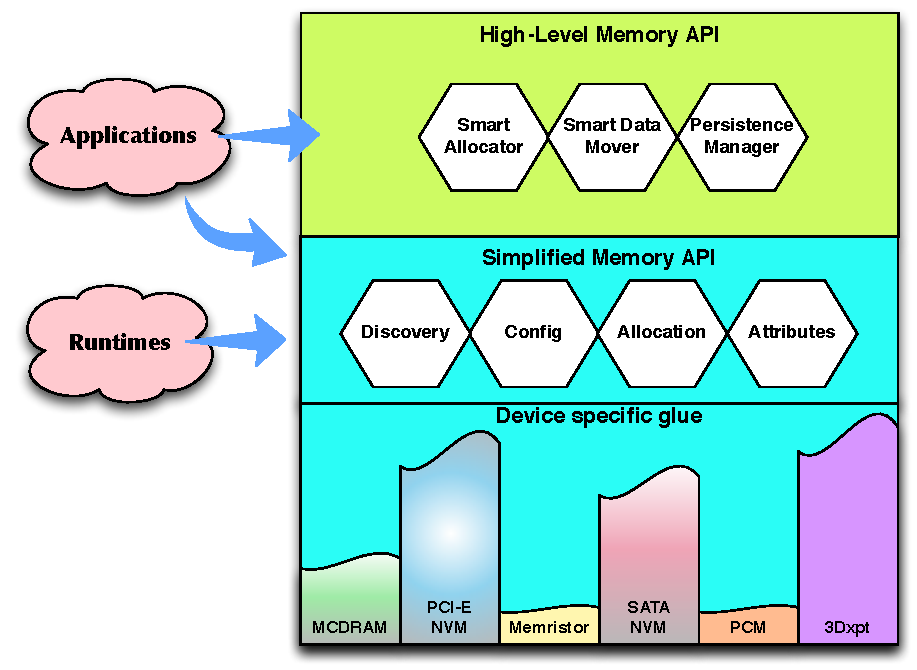
\includegraphics[width=.85\textwidth]{pres/figures/sicm.pdf}
\end{frame}

% Our Approach - Outline
\begin{frame}{Our Approach}
  \begin{customlist}{0em}{0em}
    \item \highlight{A}: Compile executable with allocation site annotations
    \item \highlight{B}: Profile memory usage of each site
    \item \highlight{C}: Generate tier recommendations
    \item \highlight{D}: Apply data tier recommendations
  \end{customlist}
  \vspace{2em}
  \centering
  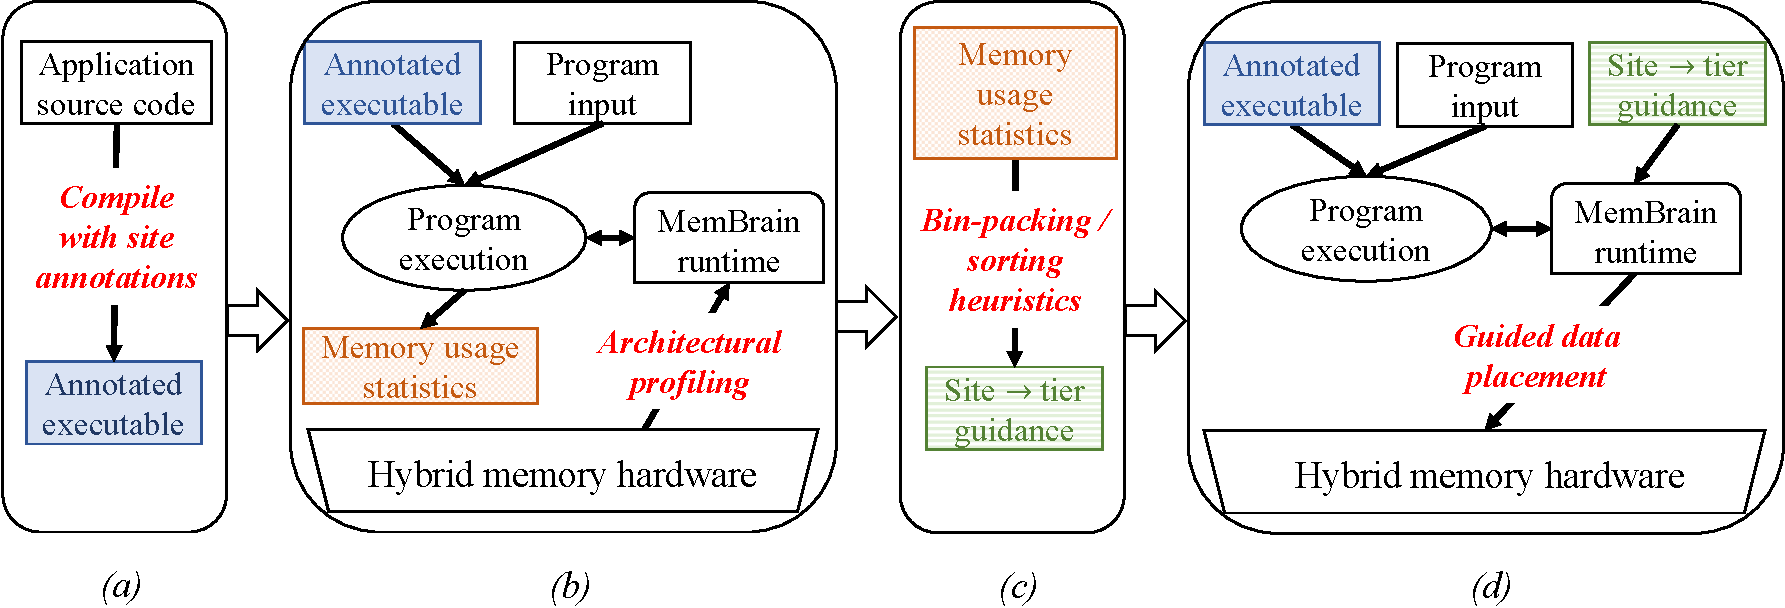
\includegraphics[width=.85\textwidth]{pres/figures/membrain.pdf}
\end{frame}

% Our Approach - Step A
\lstset{showspaces=false,showstringspaces=false}%
\defverbatim[colored]\lstI{%
  \begin{lstlisting}[language=C++,basicstyle=\ttfamily\scriptsize,
                     keywordstyle=\color{blue}\ttfamily,stringstyle=\color{red}\ttfamily,
                     commentstyle=\color{green}\ttfamily,breaklines=true]
  ptr = malloc(64);
  \end{lstlisting}
}
\begin{frame}{Annotating Allocation Sites}
  \begin{customlist}{0em}{0em}
    \item Identifies and annotates all allocation sites automatically
    \item No source code modification
    \item LLVM compiler pass
    \item Simple compiler wrappers
  \end{customlist}
  \centering
  \vspace{2em}
  \begin{tikzpicture}[>={LaTeX[width=2mm,length=2mm]},->]
    \node[draw, anchor=east] (A) {\small\texttt{ptr = malloc(64);}};
    \node[draw, right=2em of A, anchor=west] (B) {\small\texttt{ptr = sh\_alloc(12, 64);}};
    \draw[line width=0.75mm] (A) -- (B);
  \end{tikzpicture}
\end{frame}

% Arena allocation
\begin{frame}{Arena Allocation}
  \centering
  \highlight{Profiling}\\
  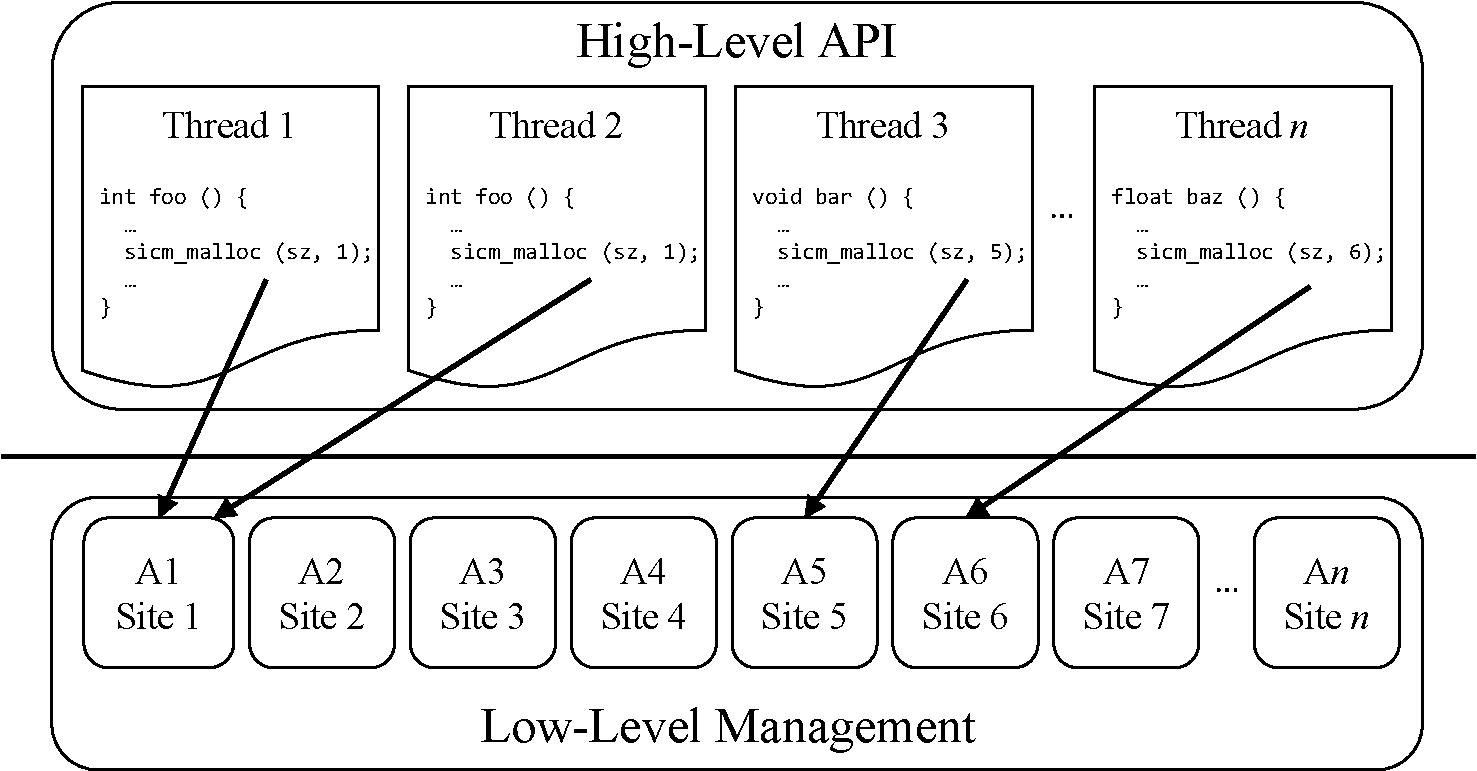
\includegraphics[width=.5\textwidth]{pres/figures/shared_sites.pdf}
  \vspace{1em}
  \noindent\rule{10cm}{0.4pt}
  \vspace{1em}\\
  \highlight{Guiding}\\
  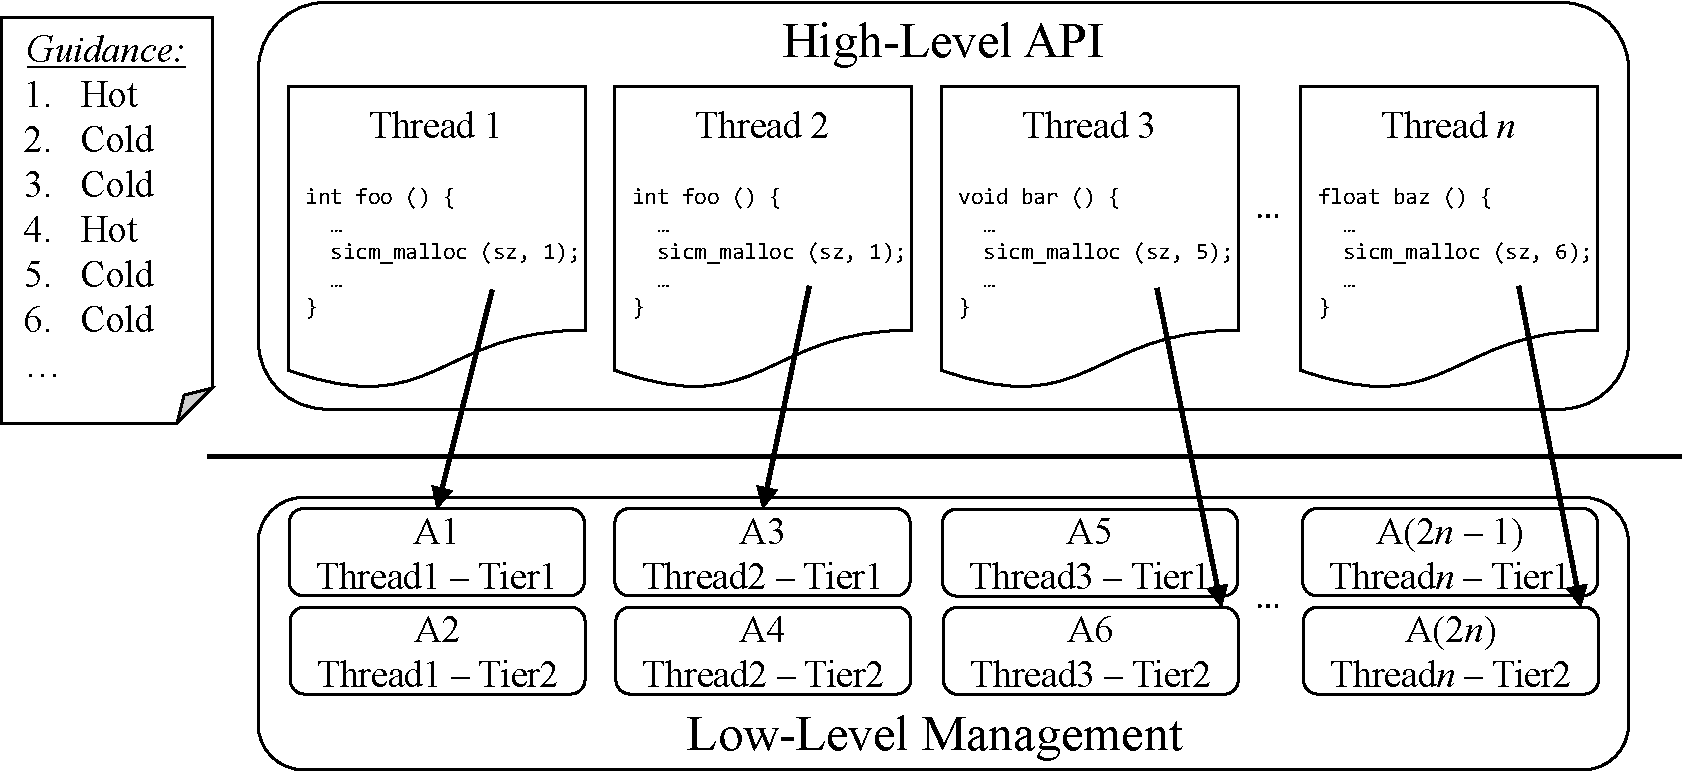
\includegraphics[width=.55\textwidth]{pres/figures/exclusive_device.pdf}
\end{frame}

% Our Approach - Step B
\begin{frame}{Profiling Memory Usage}
  \begin{customlist}{0em}{0em}
    \item Uses the \texttt{perf} interface to \highlight{PEBS}
    \item Last-level cache misses
    \item Includes logical address that was accessed, can associate with allocation site
  \end{customlist}
\end{frame}

% Our Approach - Step C
\begin{frame}[fragile]{Generating Tier Recommendations}
  \begin{customlist}{0em}{0em}
    \item \highlight{Input} is per-site profiling information
    \item \highlight{Output} is per-site tier recommendations
    \item Algorithms:
    \begin{customlist}{1em}{0em}
      \item knapsack
      \item hotset
      \item thermos
    \end{customlist}
  \end{customlist}
  \vspace{2em}
  \begin{center}
  \begin{tikzpicture}[>={LaTeX[width=2mm,length=2mm]},->]
    \node[file] (A) {\highlight{Profiling} \nodepart{second} 12 2048\\13 8192\\14 4096};
    \node[file, right=2em of A] (B) {\highlight{Guidance} \nodepart{second} 12 0\\13 1\\14 0};
    \draw[line width=0.75mm] (A) -- (B);
  \end{tikzpicture}
  \end{center}
\end{frame}

% Our Approach - Step D
\begin{frame}{Applying Tier Recommendations}
  \begin{customlist}{0em}{0em}
    \item Reads in file of tier recommendations
    \item Uses per-thread arenas for more efficient execution
    \item Uses \texttt{mbind} to bind sites to appropriate tier
  \end{customlist}
  \vspace{2em}
\end{frame}

\begin{frame}{Experiments}
  \begin{customlist}{0em}{0em}
    \item \highlight{CLX} is a Xeon "Cascade Lake" machine
    \begin{customlist}{1em}{0em}
      \item Upper tier: 192GB of DDR4
      \item Lower tier: 512GB of Optane DC DIMMs
    \end{customlist}
    \item \highlight{KNL} is a Knights Landing platform
    \begin{customlist}{1em}{0em}
      \item Upper tier: 16GB of MCDRAM
      \item Lower tier: 96GB of DDR4
    \end{customlist}
  \end{customlist}

  \vspace{1em}

  \begin{minipage}{\paperwidth}
  \begin{columns}[T,onlytextwidth]%
  \column{.3\textwidth}%
    \begin{customlist}{0em}{0em}
      \item Four workloads:
      \begin{customlist}{1em}{0em}
        \item LULESH
        \item AMG
        \item SNAP
        \item QMCPACK
      \end{customlist}
    \end{customlist}
  \column{.7\textwidth}%
    \centering
    \begin{table}[t]
      \centering
      \footnotesize
      \begin{tabular}{|c|r|r|r|r|}
        % Header
        \hline
        \multirow{2}{*}{Machine} &
        \multicolumn{4}{c|}{Size} \\
        \cline{2-5}
        & SM & MED & LG & HG \\
        \hline

        % Values
        KNL & \textasciitilde12 & \textasciitilde40 & \textasciitilde80 & N/A \\
        \hline
        CLX & \textasciitilde12 & \textasciitilde140 & \textasciitilde300 & \textasciitilde500 \\
        \hline
      \end{tabular}
    \end{table}
  \end{columns}
  \end{minipage}
\end{frame}

\begin{frame}{Profiling Overhead}
  \centering
  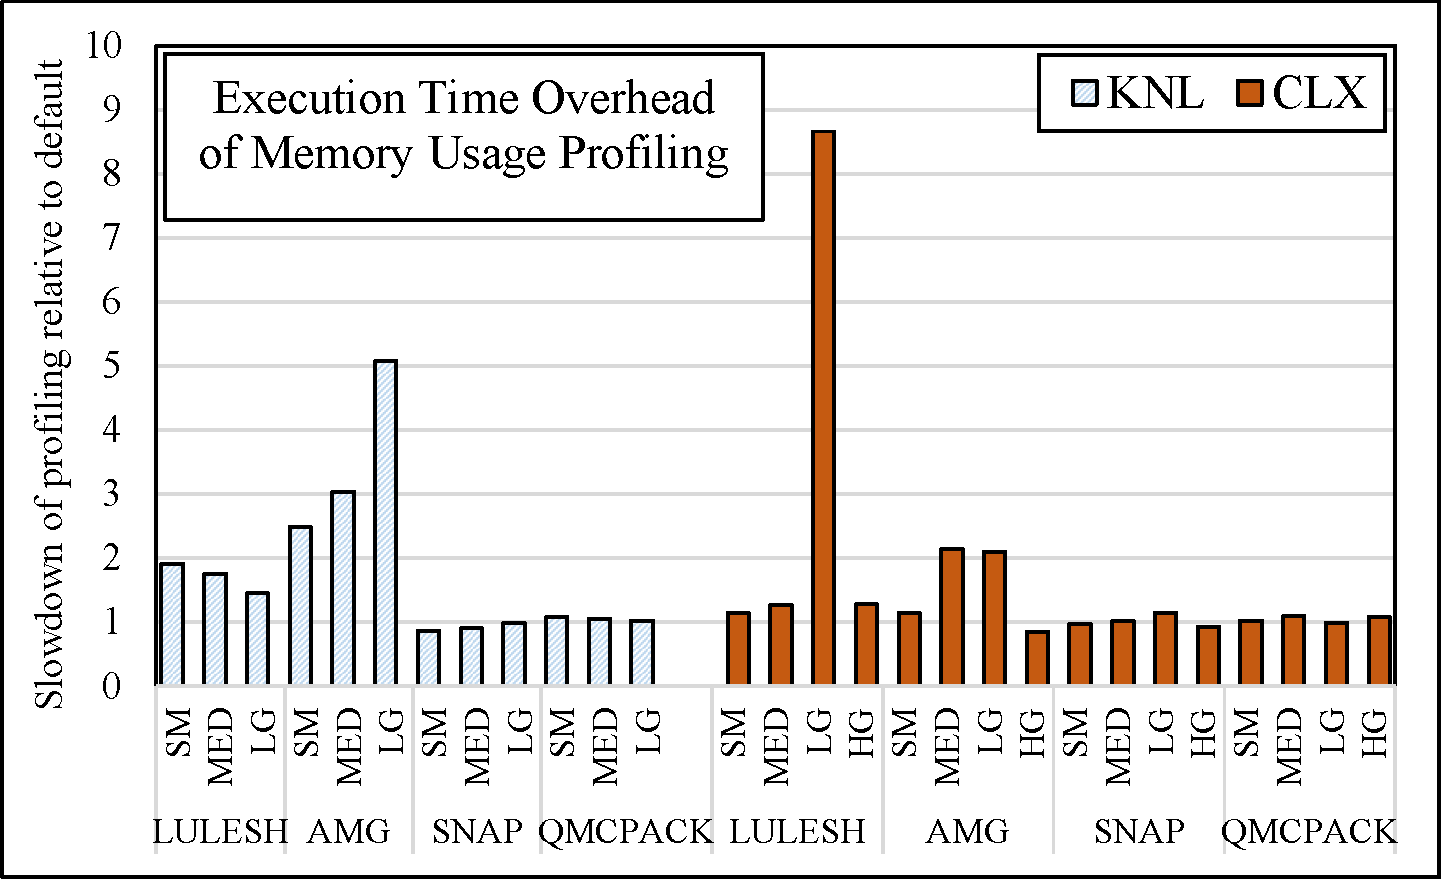
\includegraphics[width=.9\textwidth]{pres/figures/profile.pdf}
\end{frame}

\begin{frame}{Varying Capacity in the Upper Tier: KNL}
  \centering
  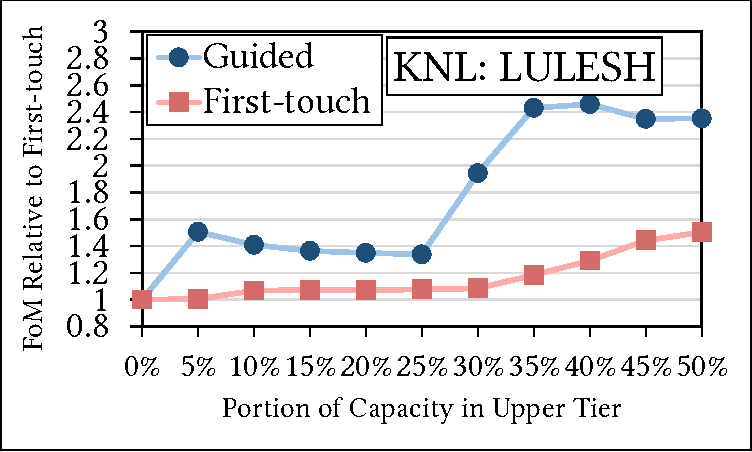
\includegraphics[width=.49\textwidth]{pres/figures/small_lulesh.pdf}
  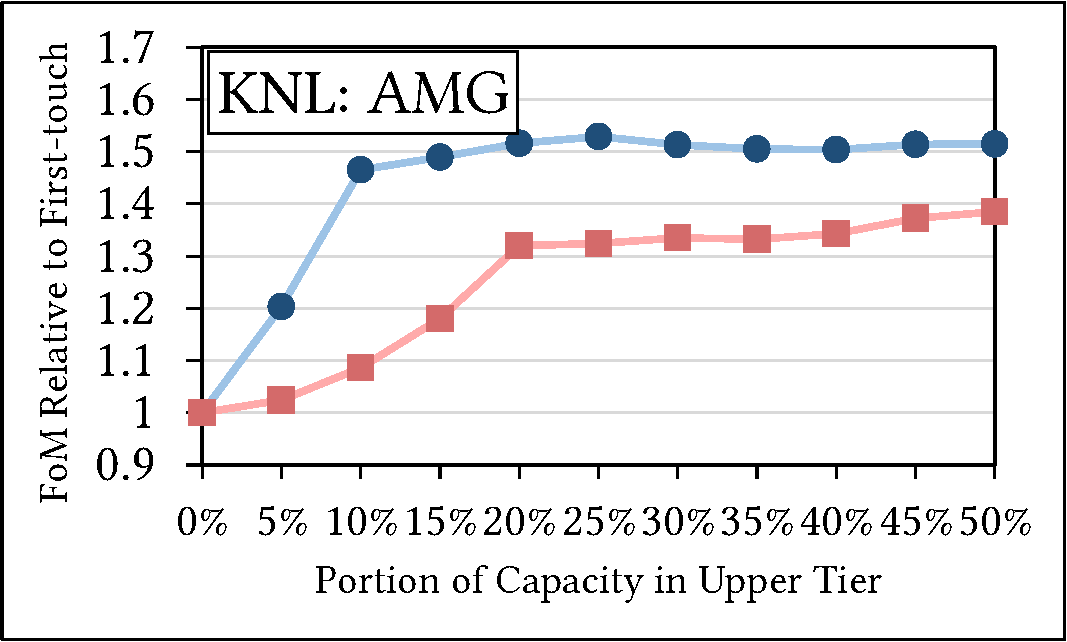
\includegraphics[width=.49\textwidth]{pres/figures/small_amg.pdf}
  \\
  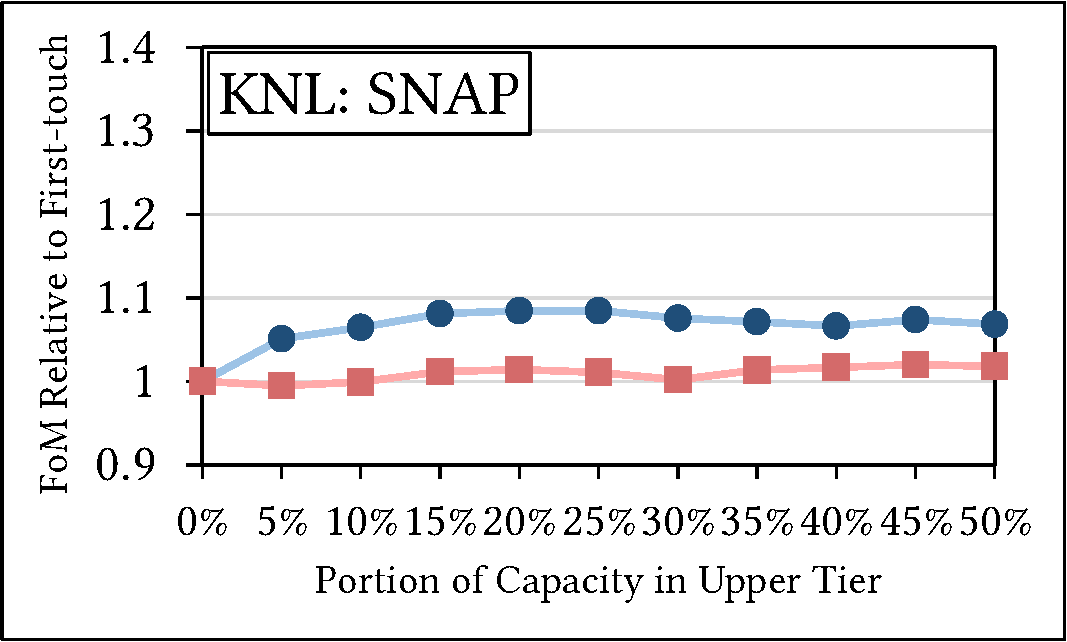
\includegraphics[width=.49\textwidth]{pres/figures/small_snap.pdf}
  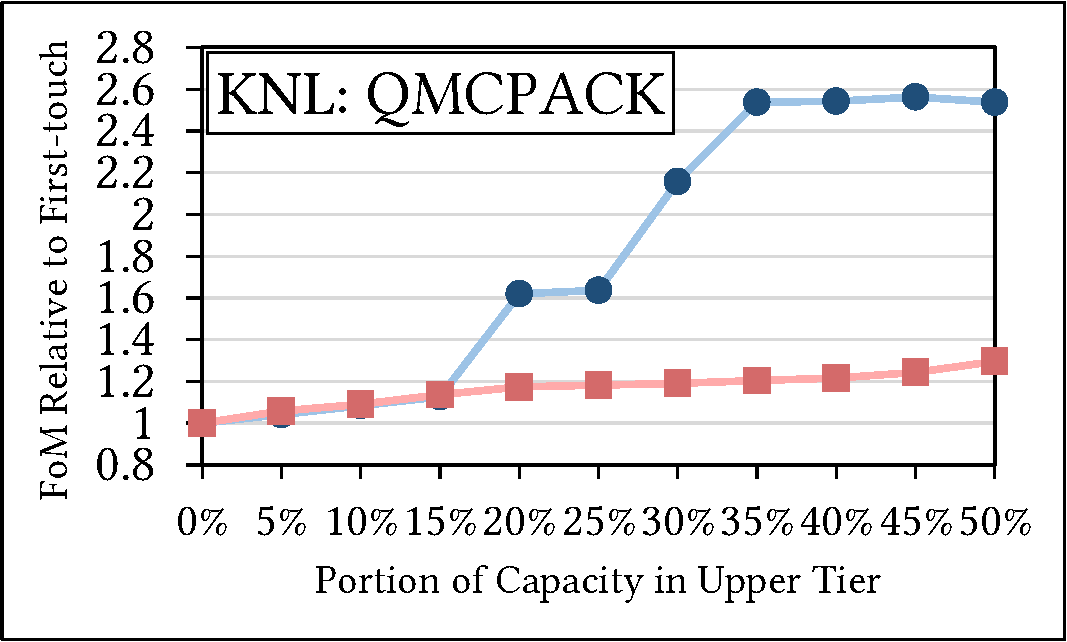
\includegraphics[width=.49\textwidth]{pres/figures/small_qmcpack.pdf}
\end{frame}

\begin{frame}{Varying Capacity in the Upper Tier: CLX}
  \centering
  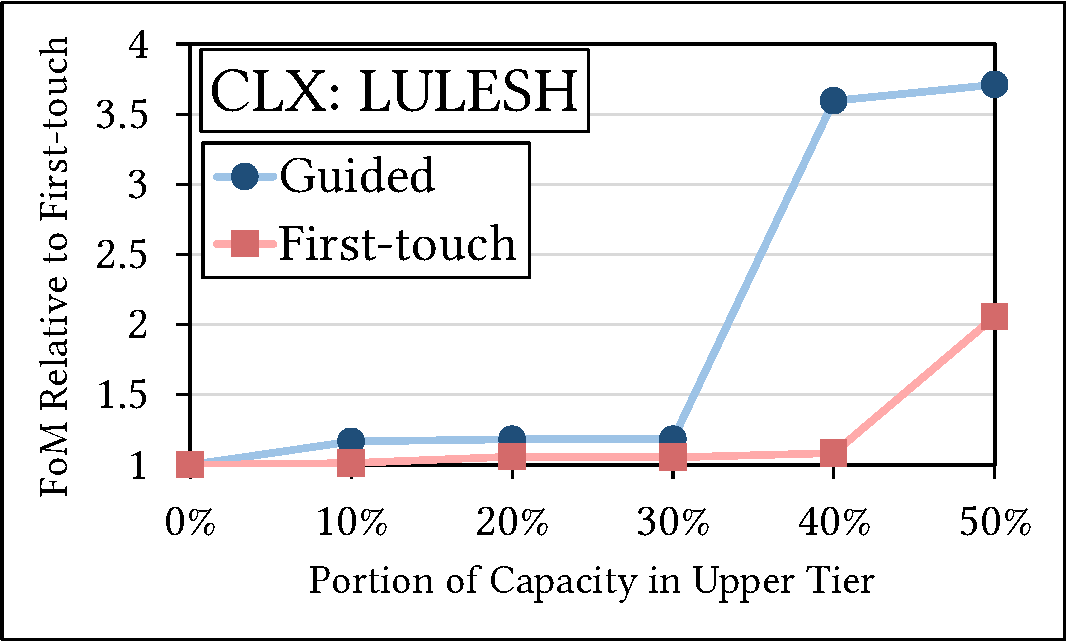
\includegraphics[width=.49\textwidth]{pres/figures/clx_small_lulesh.pdf}
  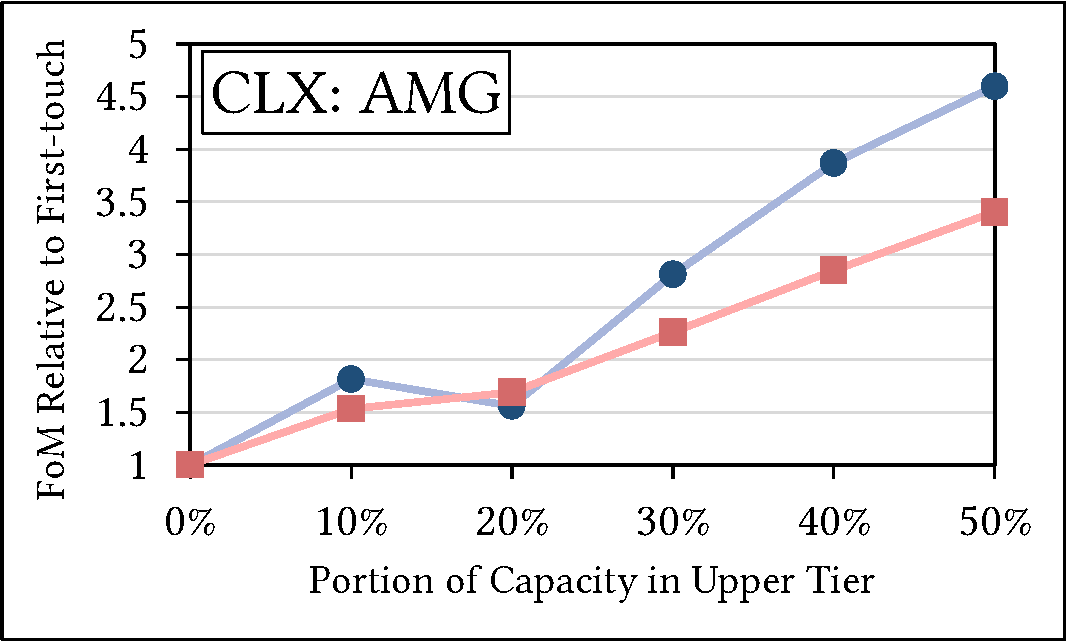
\includegraphics[width=.49\textwidth]{pres/figures/clx_small_amg.pdf}
  \\
  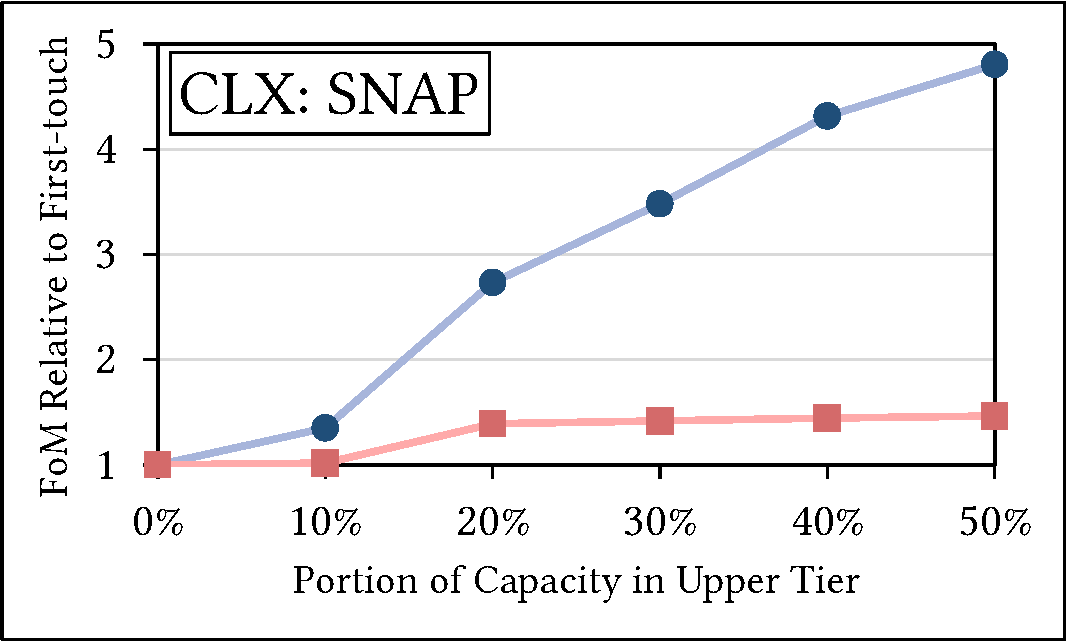
\includegraphics[width=.49\textwidth]{pres/figures/clx_small_snap.pdf}
  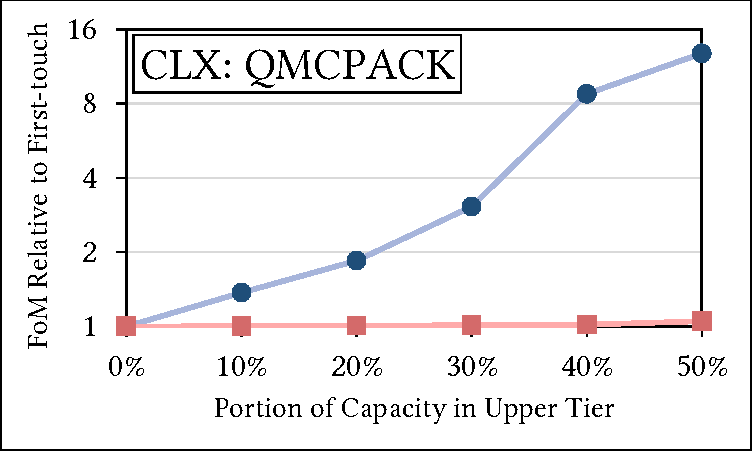
\includegraphics[width=.49\textwidth]{pres/figures/clx_small_qmcpack.pdf}
\end{frame}

\begin{frame}{Full-Sized Performance: KNL}
  \centering
  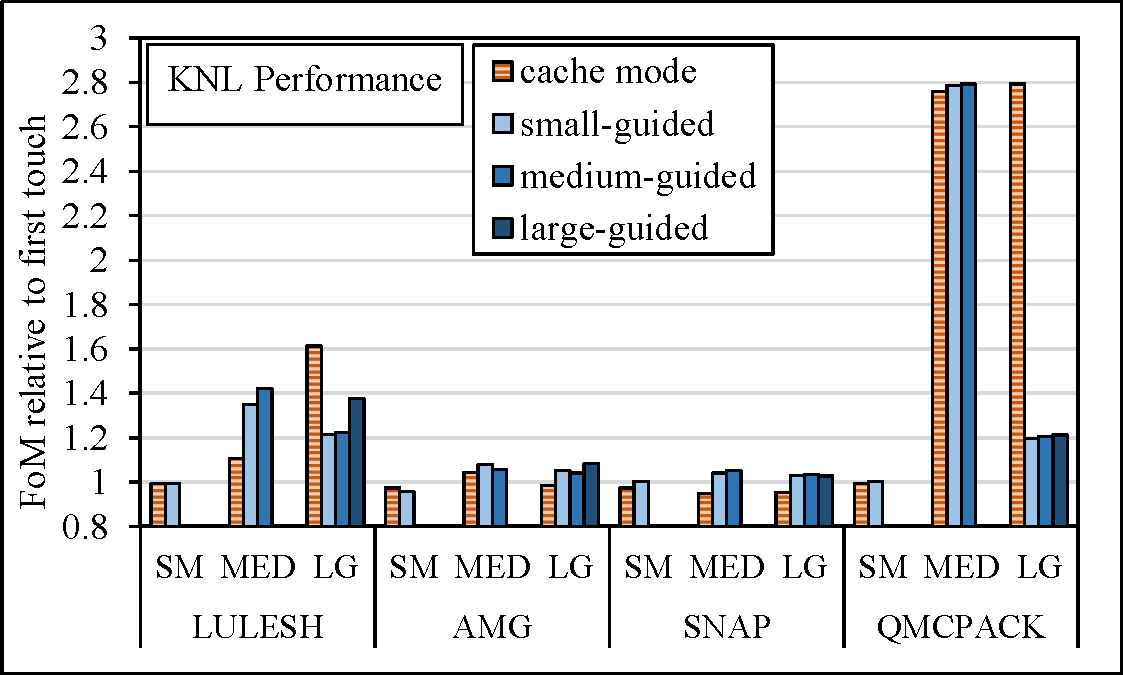
\includegraphics[width=.9\textwidth]{pres/figures/knl_perf.pdf}
\end{frame}

\begin{frame}{Full-Sized Performance: CLX}
  \centering
  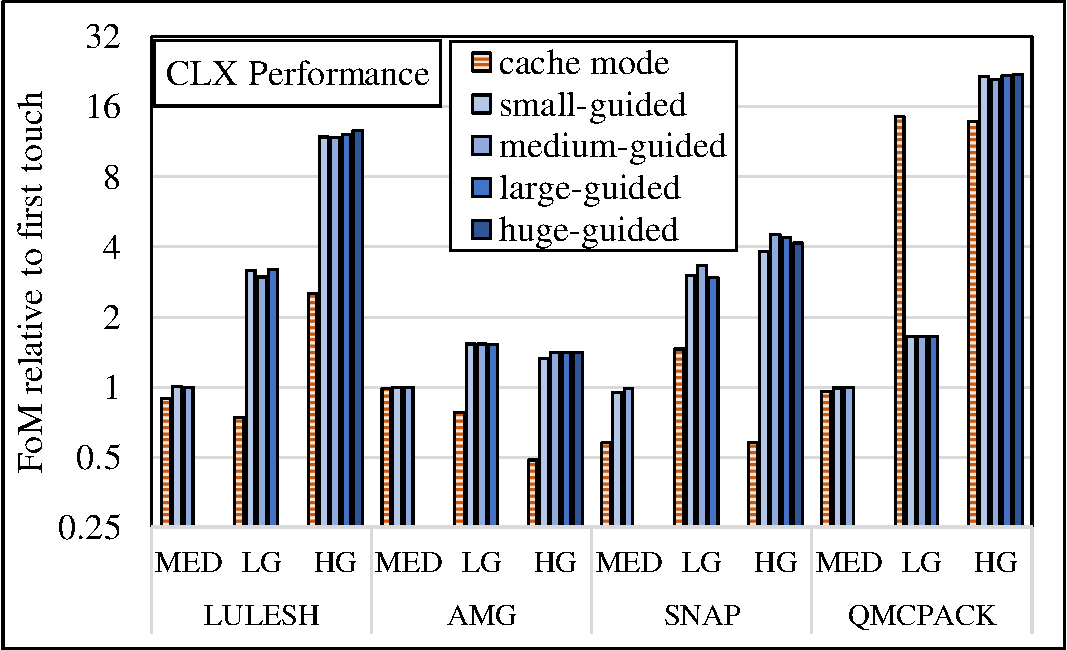
\includegraphics[width=.9\textwidth]{pres/figures/aep_perf.pdf}
\end{frame}

\begin{frame}{Cross-Platform Performance}
  \centering
  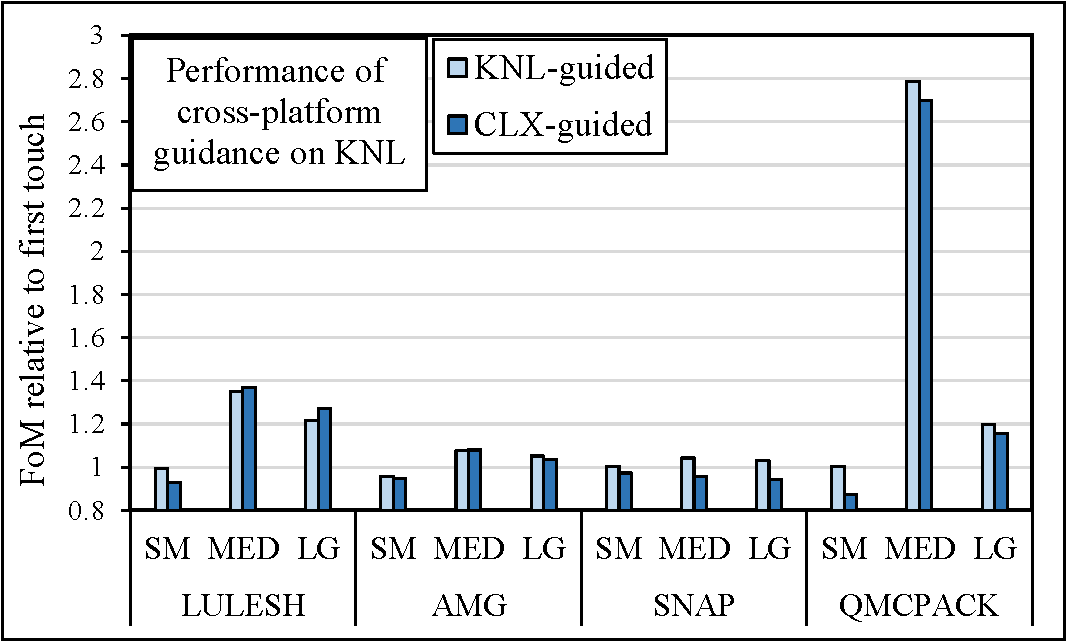
\includegraphics[width=.6\textwidth]{pres/figures/knl_cross.pdf}
  \\
  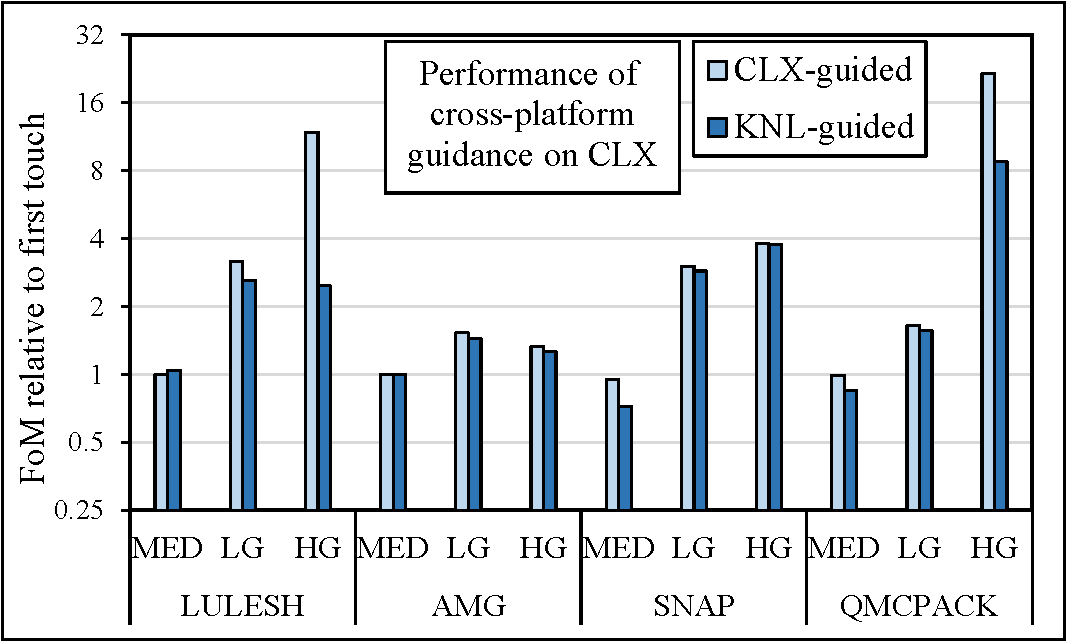
\includegraphics[width=.6\textwidth]{pres/figures/aep_cross.pdf}
\end{frame}

\end{document}
